\section{Einrichtung des ADS-Workspaces}

    \subsection{Auswahl der Technologie und Erstellung des Substrat-Files}
    Bevor wir in ADS die Leitungen Simulieren können, muss das Substrat file definiert werden.
    Hier lässt sich die dicke der Kupferleitung sowie von dem Dielektrikum FR4 wählen.
        \begin{itemize}
            \item FR4    : 1mm
            \item Kupfer : 35\textmu m
        \end{itemize}
        \begin{figure}[H]
            \centering
            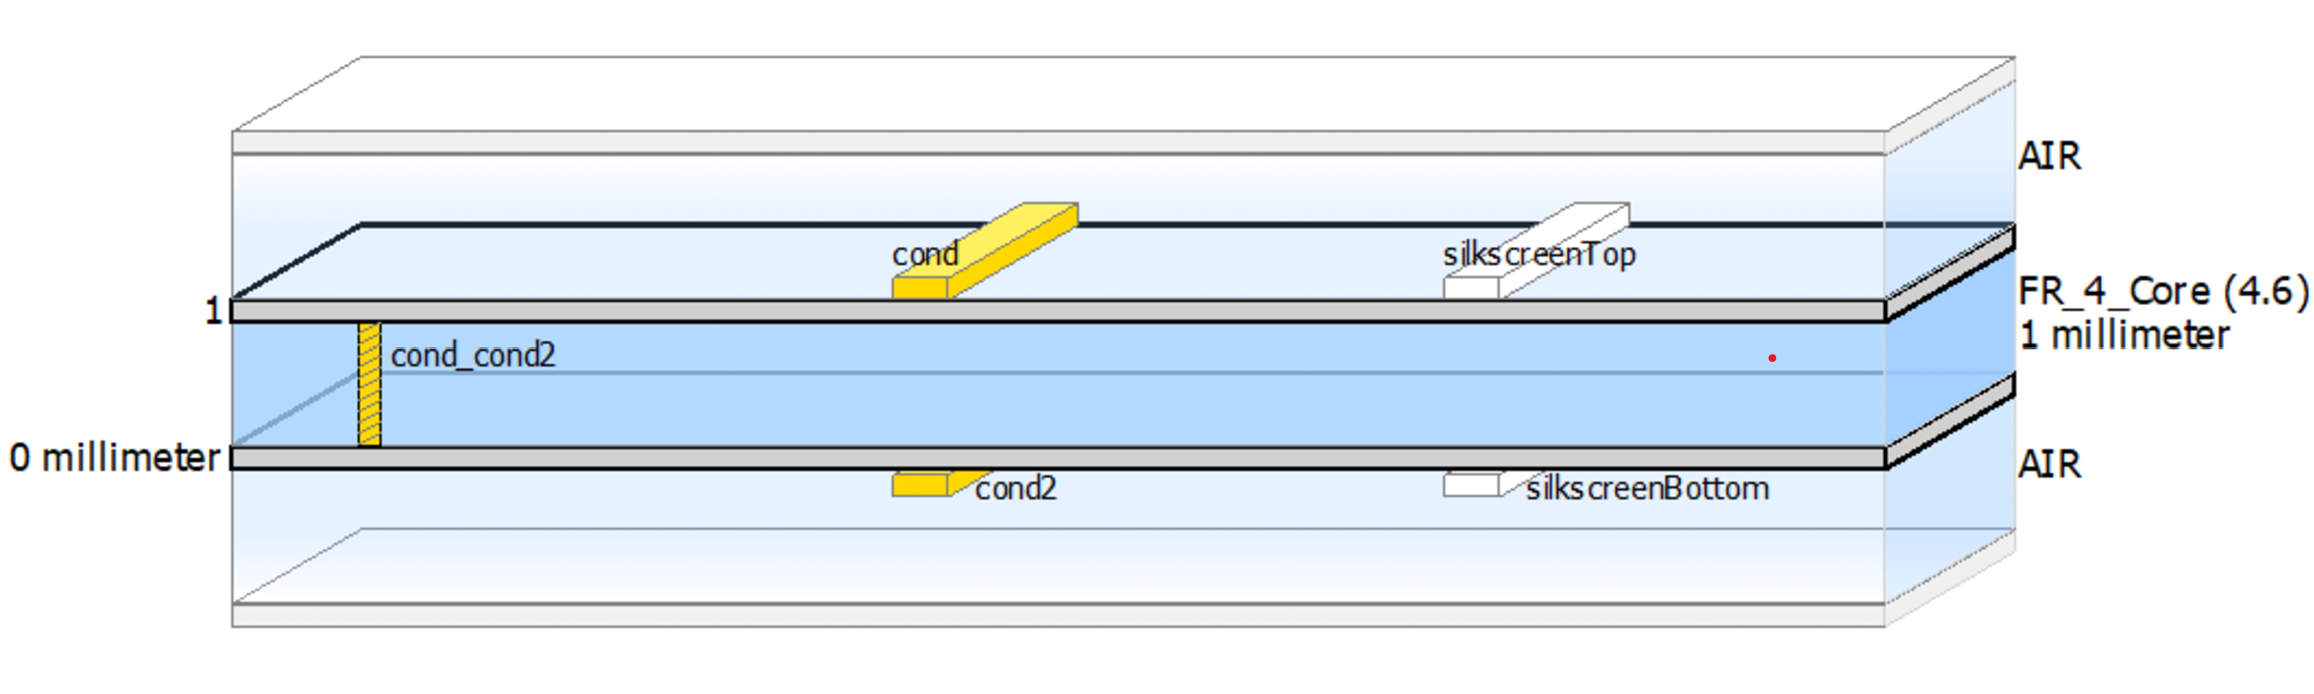
\includegraphics[width=0.9\textwidth]{Pictures/substratFile.png}
            \caption{Substratfile}
        \end{figure}

    \subsection{Nutzung des Controlled Impedance Line Designers}

\section{Leitungsdimensionierung}
    \subsection{\texorpdfstring{Berechnung der Leitungsbreite ($Z_0 = 50~\Omega$)}{Berechnung der Leitungsbreite (Z0 = 50 Ohm)}}
    Nun wird die Leitungsbreite einer Microstrip Leitung mit der Wellenimpedanz $Z_0 = 50~\Omega$ berechnet.
    Dazu verwenden wir die Formeln, die uns auf der Website von Microwaves101 Kapitel Microstrip zur
    Verfügung gestellt werden. Durch eine grobe Abmessung der Leitungsbreite sieht man das folgende Beziehung gilt: \\
    \[
    \frac{w}{h} \geq 1
    \]
    $w$ ist hier die Leitungsbreite und $h$ die Höhe des Dielektrikums. In unserem Fall ist $h = 1mm$ und $w$ wird variiert. Die 
    effektive Permitivität wird mit folgender Formel berechnet:
      \[
    \varepsilon_e = \frac{\varepsilon_r + 1}{2} + \frac{\varepsilon_r - 1}{2} \left( 1 + 12 \frac{h}{w} \right)^{-\frac{1}{2}}
    \]
   \\ $\varepsilon_e$ wird in die Formel zur Leitungsimpedanz eingesetzt. Bei dieser wird $w$
    variiert, bis die Wellenimpedanz $Z_0 = 50~\Omega$ erreicht wird.
    \\
    Die Formel zur Leistungsimpedanz $Z_o$ lautet:
    \[
    Z_0 = \frac{120 \pi}{\sqrt{\varepsilon_{\text{eff}}} \left( \frac{w}{h} + 1.393 + \frac{2}{3} \ln\left( \frac{w}{h} + 1.444 \right) \right)} \quad \text{(Ohm)}
    \]
    Die Berechnung der Leitungsbreite wird hierbei numerisch durchgeführt, da eine analytische Berechnung zu
    komplex werden würde. Die Ergebnisse der Approximation werden in Tablle 4.1 dargestellt. \\
    
    \begin{table}[H]
        \centering
        \begin{tabular}{|l|l|}
            \hline
            \textbf{Leitungsbreite $w$ (mm)} & \textbf{Wellenimpedanz $Z_0$ ($\Omega$)} \\
            \hline
            1.7 & 52.749 \\
            1.8 & 51.027 \\
            1.9 & 49.419 \\
            2.0 & 47.915 \\
           
            \hline
        \end{tabular}
        \caption{Berechnete Wellenimpedanz für verschiedene Leitungsbreiten}
    \end{table}
    Anhand der berechneten Werte liegt die Leitungsbreite mit $w = 1.8~mm$ am nähesten an der Wellenimpedanz.
    Eine nähere Berechnung ist mit unserem TR nicht möglich. 

       

    \subsection{Verifizierung der Berechneten Leitungsbreite}
    Nun wird die Leitungsbreite mithilfe des Controlled Impedance Line Designers Simuliert.
    Ziel ist es die $Z_0 = 50~\Omega$ zu erreichen durch sweepen der Leitungsbreite
    \begin{figure}[H]
        \centering
        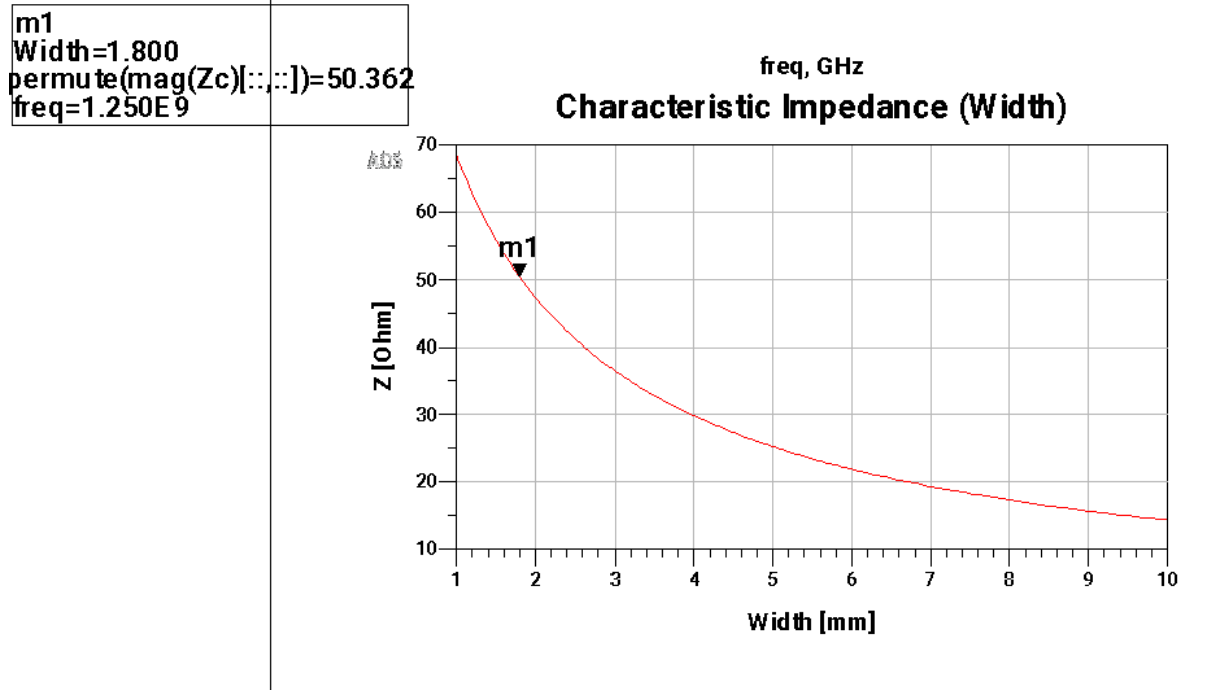
\includegraphics[width=0.8\textwidth]{Pictures/LeitungsbreitenSweep.png}
        \caption{Wellenimpedanz in abhängigkeit von der Leitungsbreite}
    \end{figure}
    Wie schon numerisch bestimmt kommen wir mitn der Leiterbreite $w=1.8mm$ der Wellenimpdanz $Z_0 = 50~\Omega$
    am nähesten. Würde man noch genauer sweepen, wird man festellen dass die Optimale Leiterbreite irgendwo zwischen
    $1.8mm$ und $1.9mm$ liegt.

    \subsection{Charakteristische Länge der Koppelleitungen}
    \subsection{Bestimmung der Filterordnung}

\section{Aufbau des Coupled-Line-Filters im Schematic}

\section{Simulation und Optimierung}
    \subsection{Vergleich mit Messdaten}

\section{Knick zur Optimierung des Aspektverhältnisses}

\section{Anpassung im Schematic und Re-Simulation}

\section{Auswirkungen auf die S-Parameter}
